\newpage
\section{UI structure}
\hspace{0.7cm} Here is the main user interface that we designed:

\vspace{1cm}
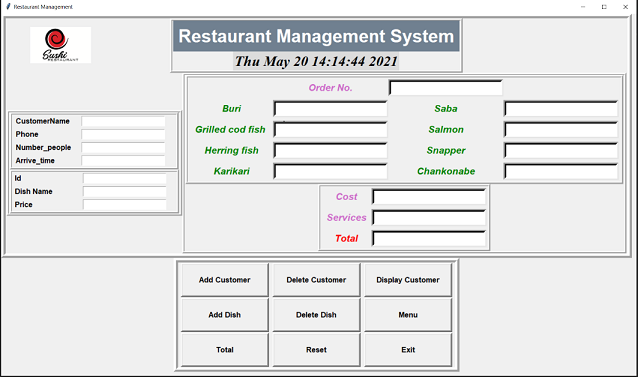
\includegraphics{images/UI structure.png}

It has three main parts: Adding, Receipt calculating and Feature buttons

\vspace{0.5cm}
\subsection{Adding}
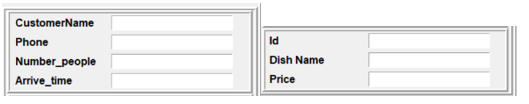
\includegraphics{images/adding.png}

\hspace{0.7cm}
In those blanks, user can enter information of either customers or dishes in order to add, delete, update or show by using the feature buttons

\newpage
\subsection{Receipt calculating}
\vspace{1cm}
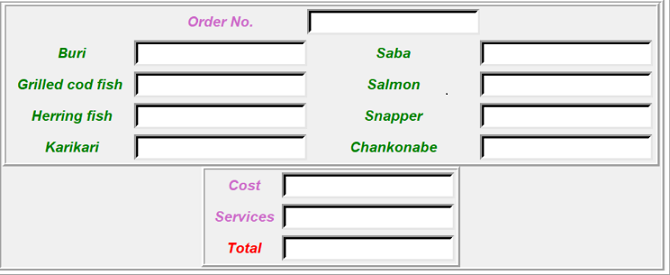
\includegraphics{images/ordering.png}

\vspace{1cm}
\textbf{This area is used to show the order of each customer}
\begin{itemize}
    \item “Order no.” part is the ID of the order. 
    \item 8 blanks under it show all the dishes the restaurant has. User can enter the quantity into it to show how many of each dish a customer ordered. 
    \item “Cost” is the price the order. 
    \item “Services” is the price of the service which equals to 10\% of the “Cost”
    \item “Total” is the total price that a customer must pay (including “Cost” and “Services”)
\end{itemize}

\newpage
\subsection{Feature buttons}
\vspace{1cm}
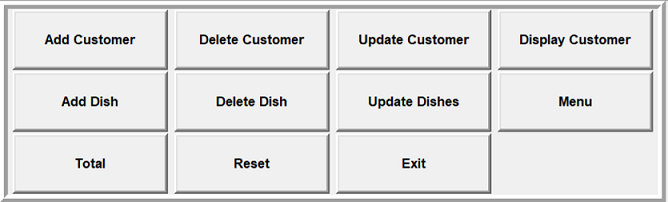
\includegraphics{images/feature button.png}

\vspace{0.5cm}
\textbf{Here is the list of all the buttons that allow users to interact with the program:}
\vspace{0.5cm}

\begin{itemize}
    \item The first row is the CRUD functions for the list of customers.
    \item The second row is the CRUD functions for the list of all the dishes.
    \item “Total” button is used to calculate the total price a customer must pay.
    \item “Reset” button’s aim is for deleting information entered in all the blank.
    \item “Exit” button is utilized to exit the program.
\end{itemize}

\subsection{Additional features}
\hspace{0.7cm} To increase the practicality and productivity of the program, we inserted some minor features to support the users. To be more precise, our program can inform people when they use it in the wrong way, validate the manager’s options, or tell the users when the tasks are done.

\vspace{1cm}
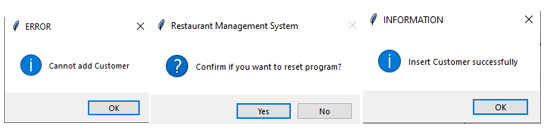
\includegraphics{images/check box error.png}